\scanpage{18}
cette dernière, si $\operatorname{card}J=\operatorname{card}I-1=n-1$, on verra (par \unsure{rècurrence|récurrence}) que le cardinal de l'ens des classes est $(n-1)+1=n$.

Ceci posé, on voit d'abord que $E_i$ est dans
% G01: full-scan origin (820,465), x right/y down; manual geometry.
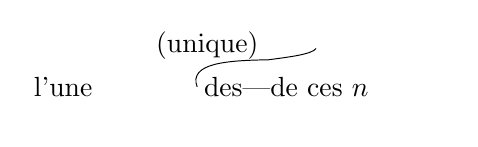
\begin{tikzpicture}[x=.08mm,y=-.08mm,baseline=(g01base)]
\path[use as bounding box] (0,0) rectangle (670,145);
\coordinate (g01base) at (0,115);
\begin{scope}[shift={(-820,-465)}]
\node[anchor=base west,inner sep=0pt,outer sep=0pt] at (830,574) {l'une};
\node[anchor=base west,inner sep=0pt,outer sep=0pt] at (1024,505) {\inserted{(unique)}};
\node[anchor=base west,inner sep=0pt,outer sep=0pt] at (1100,574) {\unsure{des|de} ces $n$};
\draw[line width=.35pt] (1089,559) .. controls (1075,521) and (1137,517) .. (1202,516) .. controls (1240,511) and (1271,507) .. (1278,498);
\end{scope}
\end{tikzpicture}
classes, qui sont des ouverts. Soit $U_{J,i}$ la classe (ou ``\unsure{composante|composant}'') qui contient $E_i$, et considérons les deux composantes $\Sigma_i^+,\Sigma_i^-$ de $X\setminus E_i$.

% G02: complete lemma group. Full-scan origin (244,1145).
% The underline and the left rule each occur once. The left rule begins
% below the first textual line; its observed endpoints are preserved.
\figure{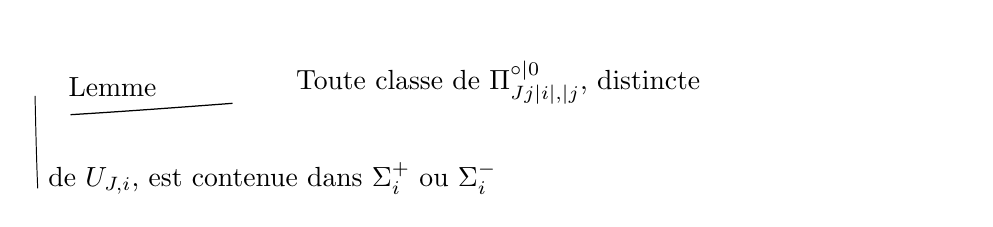
\begin{tikzpicture}[x=.085mm,y=-.085mm,baseline=(g02base)]
\path[use as bounding box] (0,0) rectangle (1400,255);
\coordinate (g02base) at (0,238);
\begin{scope}[shift={(-244,-1145)}]
\node[anchor=base west,inner sep=0pt,outer sep=0pt] at (305,1248) {\rlap{Lemme}\phantom{\uline{Lemme}}};
\node[anchor=base west,inner sep=0pt,outer sep=0pt] at (645,1238) {Toute classe de $\Pi_{J\unsure{\deleted{j}|\deleted{i}|\deleted{,}|j}}^{\unsure{\circ|0}}$, distincte};
\node[anchor=base west,inner sep=0pt,outer sep=0pt] at (275,1382) {de $U_{J,i}$, est contenue dans $\Sigma_i^+$ ou $\Sigma_i^-$};
\draw[line width=.45pt] (308,1275) .. controls (390,1270) and (471,1264) .. (550,1258);
\draw[line width=.35pt] (255,1247) .. controls (256,1290) and (257,1340) .. (259,1385);
\end{scope}
\end{tikzpicture}}

C'est presque une tautologie : Dire
% G03: whole adjoining correction group, origin (225,1465).
% The short hook after U_alpha belongs to G03b, with no separate comma.
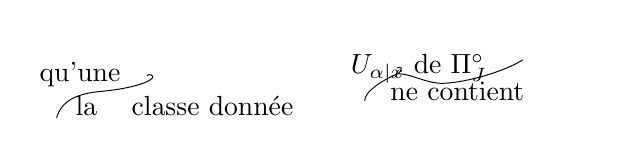
\begin{tikzpicture}[x=.08mm,y=-.08mm,baseline=(g03base)]
\path[use as bounding box] (0,-28) rectangle (925,140);
\coordinate (g03base) at (0,111);
\begin{scope}[shift={(-225,-1465)}]
\node[anchor=base west,inner sep=0pt,outer sep=0pt] at (301,1576) {\deleted{la}};
\node[anchor=base west,inner sep=0pt,outer sep=0pt] at (244,1523) {\inserted{qu'une}};
\node[anchor=base west,inner sep=0pt,outer sep=0pt] at (390,1576) {classe donnée};
\node[anchor=base west,inner sep=0pt,outer sep=0pt] at (738,1510) {\inserted{$U_{\unsure{\alpha|x}}$ de $\Pi_J^\circ$}};
\node[anchor=base west,inner sep=0pt,outer sep=0pt] at (801,1553) {ne contient};
% G03a: qu'une guide, one connected run with a hooked upper endpoint.
\draw[line width=.35pt] (271,1580) .. controls (279,1551) and (307,1541) .. (343,1538) .. controls (376,1535) and (414,1527) .. (423,1517) .. controls (426,1512) and (418,1510) .. (414,1513);
% G03b: second guide and its connected small hook, two path commands.
\draw[line width=.35pt] (760,1553) .. controls (759,1538) and (794,1517) .. (813,1510) .. controls (838,1511) and (861,1528) .. (891,1525) .. controls (938,1521) and (992,1501) .. (1011,1488);
\draw[line width=.35pt] (813,1510) .. controls (823,1501) and (817,1498) .. (811,1501);
\end{scope}
\end{tikzpicture}
pas $\deleted{\Sigma}$\begin{tikzpicture}[x=.08mm,y=-.08mm,baseline=(g04base)]
% G04: corrected E_i and the separate upper stroke. Outer origin
% (1308,1480); inner overmark origin (1324,1492), baseline y=12.
% Closure-bar/remnant role is unresolved; the visible stroke is retained
% once, including its short returning right end, under local unsure.
\path[use as bounding box] (0,0) rectangle (85,85);
\coordinate (g04base) at (0,67);
\node[anchor=base west,inner sep=0pt,outer sep=0pt] at (0,67) {$E_i$};
\node[anchor=base west,inner sep=0pt,outer sep=0pt] at (16,24) {\unsure{\begin{tikzpicture}[x=.08mm,y=-.08mm,baseline=(g04markbase)]
\path[use as bounding box] (0,0) rectangle (55,12);
\coordinate (g04markbase) at (0,12);
\draw[line width=.45pt] (0,6) .. controls (17,5) and (34,6) .. (47,6) -- (31,10) -- (43,6);
\end{tikzpicture}}};
\end{tikzpicture}
i.e. est $\ne U_{J,i}$, signifie que il existe un $j\in J$ tel que le $\Sigma_j^+\in\pi_0(X\setminus\deleted{\Sigma}E_{\unsure{j|J}})$
% G05: crossed word plus the two additional upper/right points.
% Outer origin (1408,1712); dots' fixed local origin (1569,1737).
\begin{tikzpicture}[x=.07mm,y=-.07mm,baseline=(g05base)]
\path[use as bounding box] (0,0) rectangle (190,100);
\coordinate (g05base) at (0,70);
\node[anchor=base west,inner sep=0pt,outer sep=0pt] at (0,70) {\deleted{\unsure{choisi|choisie}}};
\node[anchor=base west,inner sep=0pt,outer sep=0pt] at (161,47) {\unsure{\begin{tikzpicture}[x=.07mm,y=-.07mm,baseline=(g05markbase)]
\path[use as bounding box] (0,0) rectangle (20,22);
\coordinate (g05markbase) at (0,22);
\fill (5,16) circle[radius=1.2];
\fill (10,6) circle[radius=1.2];
\end{tikzpicture}}};
\end{tikzpicture}
``\unsure{composant|composante}'' de cette classe \deleted{est} est l'\unsure{élêment|élément} du $\pi_0$ qui ne contient pas $E_i$; il est donc contenu dans l'un des
% G06: whole éléments / (soit Sigma_i^-) / de group, origin (251,2160).
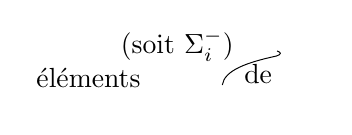
\begin{tikzpicture}[x=.08mm,y=-.08mm,baseline=(g06base)]
\path[use as bounding box] (0,0) rectangle (470,126);
\coordinate (g06base) at (0,95);
\begin{scope}[shift={(-251,-2160)}]
\node[anchor=base west,inner sep=0pt,outer sep=0pt] at (265,2255) {éléments};
\node[anchor=base west,inner sep=0pt,outer sep=0pt] at (399,2201) {\inserted{(soit $\Sigma_i^-$)}};
\node[anchor=base west,inner sep=0pt,outer sep=0pt] at (595,2248) {de};
\draw[line width=.35pt] (560,2251) .. controls (563,2228) and (599,2215) .. (646,2205) .. controls (655,2202) and (653,2199) .. (647,2197);
\end{scope}
\end{tikzpicture}
$\pi_0(X\setminus\Sigma_i)$, d'après l'étude du cas
% G07: lower correction, origin (382,2265). Actual cancellation drawn
% once; the invisible deleted copy supplies annotation/dimensions only.
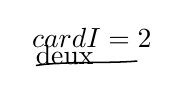
\begin{tikzpicture}[x=.08mm,y=-.08mm,baseline=(g07base)]
\path[use as bounding box] (0,0) rectangle (190,80);
\coordinate (g07base) at (0,59);
\begin{scope}[shift={(-382,-2265)}]
\node[anchor=base west,inner sep=0pt,outer sep=0pt] at (395,2323) {\rlap{\unsure{deux}}\phantom{\deleted{\unsure{deux}}}};
\node[anchor=base west,inner sep=0pt,outer sep=0pt] at (389,2297) {\inserted{$\operatorname{card}I=2$}};
\draw[line width=.55pt] (395,2325) .. controls (443,2318) and (509,2322) .. (556,2318);
\end{scope}
\end{tikzpicture},
\deleted{\unsure{OK|cela|et}} \unsure{â|à} fortiori $U_\alpha\subset\Sigma_i^-$,
% G08: final OK and its rising transverse stroke, origin (1450,2255).
% Whole-state candidates: live OK; deleted OK. The local unsure retains
% this unresolved state; no extra generic cancellation line is drawn.
\unsure{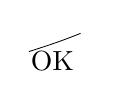
\begin{tikzpicture}[x=.08mm,y=-.08mm,baseline=(g08base)]
\path[use as bounding box] (0,0) rectangle (95,85);
\coordinate (g08base) at (0,70);
\begin{scope}[shift={(-1450,-2255)}]
\node[anchor=base west,inner sep=0pt,outer sep=0pt] at (1455,2323) {\rlap{OK}\phantom{\deleted{OK}}};
\draw[line width=.3pt] (1452,2293) .. controls (1470,2287) and (1497,2279) .. (1534,2264);
\end{scope}
\end{tikzpicture}}.
% archive sheet number: 17
